%\usepackage{extsizes}
\documentclass[14pt, a4paper, russian]{report}

\linespread{1.3}

\usepackage{titlesec}
\usepackage[centertags]{amsmath}
\usepackage{amsthm,amsfonts,amssymb}
\usepackage{indentfirst}

\usepackage{extsizes}
\usepackage[left=25mm,right=10mm,top=20mm,bottom=20mm,bindingoffset=0cm]{geometry}

\usepackage{cmap}
\usepackage{multirow}
\usepackage{float}


% \usepackage{jmlda}
% \usepackage{amsmath}

\usepackage[T2A]{fontenc}
\usepackage[utf8]{inputenc}
\usepackage[english,russian]{babel}
%\usepackage{pscyr}
\RequirePackage{graphicx}
\RequirePackage{subfig}
\RequirePackage{pgfplots}
\usepackage{thmtools}   
\usepackage{hyperref}
\usepackage[nameinlink]{cleveref}


\newtheorem{lemma}{\indent Лемма}
\newtheorem{theorem}{\indent Теорема}
\newtheorem{corollary}{\indent Следствие}
\newtheorem{problem}{\indent Задача}
\newtheorem{remark}{\indent Замечание}
\newtheorem{definition}{\indent Определение}
\newtheorem{proposition}{\indent Утверждение}
\newtheorem{example}{\indent Пример}
\newtheorem{notation}{\indent Обозначение}

\crefname{lemma}{л.}{л.}
\crefname{theorem}{теор.}{теор.}
\crefname{corollary}{след.}{след.}
\crefname{definition}{опр.}{опр.}
\crefname{proposition}{утв.}{утв.}
\crefname{example}{прим.}{прим.}
\crefname{notation}{обозн.}{обозн.}

\crefname{theorem}{Теорема}{Теорема}
\newcommand{\order}[2]{#1_{(#2)}}

\newcommand{\T}{^{\text{\tiny\sffamily\upshape\mdseries T}}}

\graphicspath{{./img/}}


\def\XYtext(#1,#2)#3{\rlap{\kern#1\lower-#2\hbox{#3}}}

% Переопределение вставки графики
\newcounter{PictureNo}

\hyphenpenalty 100
\tolerance 10000


\newenvironment{Proof}%
    {\par\noindent{\bf Доказательство.}}%
    {\hfill$\scriptstyle\blacksquare$}

\usepackage{bbm}
\bibliographystyle{unsrt}

\addto\captionsenglish{\renewcommand{\figurename}{Рисунок}}
\addto\captionsenglish{\renewcommand{\tablename}{Таблица}}
\captionsetup[figure]{labelfont=footnotesize,textfont=footnotesize}
\captionsetup[table]{labelfont=footnotesize,textfont=footnotesize}

\addto\captionsenglish{\renewcommand{\proofname}{Доказательство}}

\makeatletter % эта строка НЕОБХОДИМА!
\renewcommand{\@chapapp}{Глава} 
\addto\captionsenglish{% Replace "english" with the language you use
  \renewcommand{\contentsname}%
    {Оглавление}%
}

\titleformat{\chapter}[display]
{\normalfont\bfseries\center}
{Глава \thechapter. }{0em}{}

\titleformat{\section}[block]
{\normalfont\bfseries\center}
{\thesection. }{0em}{}

\makeatletter
\newcommand*{\indep}{%
  \mathbin{%
    \mathpalette{\@indep}{}%
  }%
}
\newcommand*{\@indep}[2]{%
  % #1: math style
  % #2: empty or \not
  \sbox0{$#1\perp\m@th$}%        box 0 contains \perp symbol
  \sbox2{$#1=$}%                 box 2 for the height of =
  \sbox4{$#1\vcenter{}$}%        box 4 for the height of the math axis
  \rlap{\copy0}%                 first \perp
  \dimen@=\dimexpr\ht2-\ht4-.2pt\relax
      % The equals symbol is centered around the math axis.
      % The following equations are used to calculate the
      % right shift of the second \perp:
      % [1] ht(equals) - ht(math_axis) = line_width + 0.5 gap
      % [2] right_shift(second_perp) = line_width + gap
      % The line width is approximated by the default line width of 0.4pt
  \kern\dimen@
  {#2}%
      % {\not} in case of \nindep;
      % the braces convert the relational symbol \not to an ordinary
      % math object without additional horizontal spacing.
  \kern\dimen@
  \copy0 %                       second \perp
} 
\newcommand{\SymPol}[2]{\overset{o}{P}{}^{#1}_{#2}}

\begin{document}
\begin{center}
\hfill \break
\footnotesize{Федеральное государственное автономное образовательное учреждение 
высшего образования}\\ 
\small{\textbf{<<Московский физико-технический институт (государственный университет)>>}}\\
\hfill \break
\normalsize{Факультет инноваций и высоких технологий}\\
\normalsize{Кафедра дискретной математики}\\
\end{center}
\footnotesize{\textbf{Направление подготовки:} 03.03.01 Прикладные математика и физика}\\
\hfill \break
\hfill \break
\hfill \break
\hfill \break
\begin{center}
\large{\textbf{Комбинаторные свойства обобщённых автоморфизмов Шакона}}\\
\normalsize{Бакалаврская работа}\\
\hfill \break
\hfill \break
\end{center}
 
\hfill \break
 
\begin{flushright}
\footnotesize{ 
\begin{tabular}{rl}
\textbf{Обучающийся:} & Слюсарев Владислав Владимирович \\
 & \underline{\hspace{3cm}} \\\\
\textbf{Научный руководитель:} & к. ф.-м. н., старший преподаватель\\
            & А. А. Приходько \\
 & \underline{\hspace{3cm}} \\\\
\end{tabular}
}
\end{flushright}

\hfill \break
\hfill \break
\hfill \break
\hfill \break
\hfill \break
\hfill \break
\begin{center} Москва 2018 \end{center}
\thispagestyle{empty} % выключаем отображение номера для этой страницы
 
% КОНЕЦ ТИТУЛЬНОГО ЛИСТА
 
\newpage

\tableofcontents{}

\chapter*{Введение}


Lorem ipsum dolor sit amet, consectetur adipiscing elit. Etiam mauris eros, venenatis id nisi ac, scelerisque dapibus metus. Aliquam scelerisque vulputate justo. Nunc ut commodo mauris. Etiam scelerisque sapien ac nisl euismod auctor. Sed eu commodo tortor, nec aliquam nulla. Nullam convallis, tellus sit amet porttitor vestibulum, orci metus sollicitudin mauris, at eleifend erat arcu et mauris. Donec vel tincidunt massa. Sed et consectetur neque. Integer libero eros, accumsan id congue ac, facilisis eu purus. Suspendisse potenti. Nullam blandit quis erat tempor ullamcorper. Suspendisse consequat condimentum turpis, et tempor lectus vulputate sed.

Nam in enim vel tortor congue cursus ac nec felis. Sed commodo arcu lorem, id gravida erat pulvinar id. Praesent maximus nisi ac ipsum malesuada tempus. Aliquam pellentesque in mi eu sagittis. Curabitur vitae quam risus. Ut sed erat auctor, pellentesque nulla eu, aliquam massa. Nunc laoreet enim velit, ut gravida odio tempus eget. Morbi nec congue libero, tincidunt vestibulum urna. Nulla sed lacus id arcu accumsan interdum. Suspendisse ut pharetra sem.

Aliquam erat volutpat. Etiam nec egestas velit. Curabitur eu metus ultricies magna cursus maximus. Proin nec eleifend ipsum. Nunc pulvinar nulla nisl, id finibus nunc faucibus eu. Cras libero magna, viverra eget eros non, fermentum tincidunt justo. Curabitur rhoncus felis lectus, ut tempus lectus congue at.

Sed tristique mauris a auctor egestas. Lorem ipsum dolor sit amet, consectetur adipiscing elit. Fusce accumsan aliquam porttitor. Fusce aliquam ante eu leo porttitor, vitae interdum dolor laoreet. Donec eget volutpat odio. Curabitur non massa tellus. Nullam in viverra mi, in hendrerit augue. Aenean vehicula dignissim elit, et condimentum mi facilisis eget. Interdum et malesuada fames ac ante ipsum primis in faucibus. Duis fermentum libero quis dapibus luctus. Sed eleifend ullamcorper sem, a tempor nunc consectetur eget. Curabitur ultrices posuere mollis. Donec iaculis leo id neque placerat, nec gravida sem venenatis. Nam elit augue, tristique vel rhoncus quis, aliquet dictum quam.

Aliquam risus sem, interdum vitae sodales sit amet, sollicitudin ut dui. Vivamus ut nisi congue, ultricies ante id, vehicula metus. Morbi eu sem id metus tincidunt tincidunt quis non libero. Vivamus at diam quis felis ullamcorper suscipit ac id turpis. In egestas id velit sit amet maximus. Sed a laoreet ligula, rhoncus ultrices dui. Integer nunc est, bibendum a consectetur eu, condimentum sit amet leo. Nulla facilisi. Nulla a ex ac mauris ultricies fermentum quis non tellus. Quisque lacinia sapien ac dui semper rutrum vitae ac velit. 

\newpage

\chapter{Основные определения}

\section{Основные обозначения и определения}

Пусть $p \ge 3$ --- произвольное натуральное число. Рассмотрим аддитивную группу вычетов $\mathbb{Z}_p$. 

\begin{definition}
Пространством $\Gamma$ назовём множество бесконечных последовательностей элементов из $\mathbb{Z}_p$:
$$\Gamma := \left\{x = \left(x_0, x_1, x_2, \ldots \right), x_k \in \{0, 1, \ldots, p - 1\} \right\}$$
Элементы $x_0, x_1, x_2, \ldots$ будем называть координатами элемента $x$.
\end{definition}
Далее мы также будем использовать множество 
$$\Gamma' := \Gamma \setminus \{(p-1,p-1,\ldots)\},$$
в котором каждая последовательность имеет в начале лишь конечное число элементов, равных $(p-1)$.

Отметим, что $\Gamma$ с операцией покоординатного сложения с переносом является компактной группой. Пусть $\lambda$ --- мера Хаара на группе $\Gamma$. Эта мера позволяет задать вероятностное пространство $(\Gamma, \mathcal{B}(\Gamma), \lambda)$.

\begin{notation} 
Пусть $a, b \in \mathbb{N},\ a \le b$ Множество $\{a, a+1, \ldots, b-1, b\} \subset \mathbb{N}$ будем называть отрезком и обозначать $\left[a, b\right]$. Учитывая естественное вложение $\mathbb{Z}_p$ в $\mathbb{N}$, мы будем использовать то же обозначение для соответствующего подмножества $\mathbb{Z}_p$, не оговаривая это особо в тех случаях, когда смысл данного обозначения читается однозначно.
\end{notation}

Относительно меры $\lambda$ все координаты $x_k, k \ge 0,$ являются независимыми одинаково распределёнными случайными величинами, имеющими дискретное равномерное распределение на множестве $\left[0, p-1\right]$. 

\begin{definition} Определим два преобразования, действующих на пространстве $\Gamma$ и сохраняющих меру $\lambda$:
\begin{itemize}
\item Преобразование сдвига на одну позицию влево $\sigma$: $x=\left(x_0, x_1, x_2, \ldots \right) \mapsto \sigma x = \left(x_1, x_2, \ldots \right)$
\item Преобразование <<прибавления единицы>> $S$: $x \mapsto x + 1$, где $1:=(1,0,0,\ldots) \in \Gamma'$, где сложение понимается в смысле групповой операции на $\Gamma$. 
\end{itemize}
\end{definition}
\begin{example}
Для иллюстрации действия этих преобразований зафиксируем $p=4$. 
\begin{itemize}
\item $\sigma (0,1,0,0,\ldots) = (1, 0, 0, \ldots)$
\item $S(1,0,0,\ldots) = (2,0,0,\ldots)$
\item $S(3,1,0,0,\ldots) = (0,2,0,0,\ldots)$
\item $S(3,3,3,2,1,1,\ldots)=(0,0,0,3,1,1,\ldots)$
\end{itemize}
\end{example}

Каждое целое число $j \ge 0$ можно отождествить с элементом множества $\Gamma'$: этот элемент получается при записи числа $j$ в системе счисления с основанием $p$ от младшего разряда к старшему с добавлением бесконечной последовательности нулей за последним знаком. Например, при $p=3$ мы отождествим число $42$ и элемент $(0,2,1,1,0,0,\ldots) \in \Gamma'$. Это обозначение согласовано с описанной выше операцией прибавления, так что мы можем говорить о прибавлении произвольного натурального числа к элементу $\Gamma'$: $S^j x = S(S(\ldots S(x)\ldots)) = x + j$ для любых $x \in \Gamma',\ j \ge 0$.

Преобразование $S^j$ является биективным для любого $j \ge 0$, поэтому мы можем говорить об обратном преобразовании $(S^j)^{-1} =: S^{-j}$. Аналогично предшествующему рассуждению, отождествим действие оператора $S^{-j}$ и вычитанию числа $j$: $S^{-j} x = x - j$.

\begin{definition}\label{phi}
Определим функционал $\phi: \Gamma' \to \mathbb{Z}$, возвращающий первую отличную от $(p-1)$ координату своего аргумента:
 \[\phi(x):=x_i\text{, если }x=(p-1, \ldots, p-1, x_i, x_{i+1}, \ldots)\]
\end{definition}
 Используя это определение, мы также определим семейство функционалов $\phi^{(m)}: \Gamma' \to \mathbb{Z},\ m \ge 0$:
\begin{definition}\label{phi_m}
    \[\phi^{(0)}(x):=0;\ \phi^{(m)}(x):=\phi(x)+\phi(Sx)+\ldots+\phi(S^{m-1}x)\]
\end{definition}
\begin{remark}
В определнии этих функционалов вычеты из $\mathbb{Z}_p$ естественным образом отождествляются с целыми числами. Таким образом, в определении $\phi^{(m)}(x)$ сложение осуществляется в множестве целых чисел, а не в группе вычетов.
\end{remark}

\begin{notation}
Пусть $n \ge 0$. Будем обозначать $\Delta_n := \sum\limits_{k=0}^{n}k = \frac{n(n+1)}{2}$. Положим также $\Delta_{-1} = 0$.
\end{notation}

\begin{example}\label{phi_delta}
Пусть $x = (x_0, x_1, \ldots) \in \Gamma'$ и $0 \le x_0 < p-1$. Если $0 < m \le p-1-x_0$, то $$\phi^{(m)}(x) = x_0 + (x_0 + 1) + \ldots + (x_0 + m - 1) = mx_0 + \Delta_{m-1}$$
Отметим, что при $m=0$ конечная формула также верна.
\end{example}

Заметим, что $\phi^{(m)}(x)$ является случайной величиной относительно пространства $(\Gamma, \mathcal{B}(\Gamma), \lambda)$, принимающей значения в $\mathbb{Z}$. Одним из основных объектов, рассматриваемых в настоящей работе, является эта случайная величина и её распределение $\pi_m$.
\begin{definition}\label{pi_m}
Пусть $j \in \mathbb{Z}$, тогда $\pi_m(j)=\lambda(\phi^{m}(x)=j)$ --- функция вероятности случайной величины $\phi^{(m)}$.
\end{definition}
\begin{example}\label{pi_example}
Легко видеть, что:
\begin{itemize}
\item $\pi_0(j) = \begin{cases}
1, & j = 0\\
0, & \text{иначе}
\end{cases}$
\item $\pi_1(j)=\begin{cases}
\frac{1}{p-1},& 0 \le j \le p-2 \\
0, & \text{иначе}
\end{cases}$
\end{itemize} 
\end{example}

При фиксированном $p$ распределения $\pi_m$ порождают семейство характеристических полиномов $P_m^p(t)$.

\begin{definition}\label{poly}
Зафиксируем натуральное число $p \ge 3$, тогда для любого целого $m \ge 0$ определим формальный полином $P_m^p(t):= \mathbb{E}_\lambda\left[ t^{\phi^{(m)}(x)}\right] = \sum\limits_{j=0}^m \pi_m(j) t^j$.
\end{definition}

Данные полиномы, рассматриваемые как семейство с параметром $m$ при фиксированном $p$, являются центральным предметом изучения в настоящей работе.

\begin{example}\label{poly_example}
Мы можем сразу вычислить первые два полинома для каждого $p$, пользуясь определением и результатами \cref{pi_example}:
\begin{equation}\label{eq:p_0}
P_0^p(t) = 1
\end{equation}
\begin{equation}\label{eq:p_1}
P_1^p(t) = \frac{1}{p-1} \sum\limits_{j=0}^{p-2} t^j
\end{equation}
\end{example}

\section{Обобщённый автоморфизм Шакона}

Зафиксируем произвольное $p \ge 3$. Определим последовательность высот $\{h_n\}_{n \ge 0}$ при помощи рекуррентного соотношения:
$$\begin{cases}
h_0 = 1 \\
h_n = p h_{n-1}+\Delta_{p-2},& n > 0 
\end{cases}$$

Для каждого $n \ge 0$ определим пространство
$$X_n:=\{(x,i): x \in \Gamma',\ 0 \le i \le h_{n-1} + \phi(x)\}$$

Рассмотрим преобразование $T_n$ пространства $X_n$, определяемое по правилу
$$T_n(x, i) := \begin{cases}
(x,i+1), & \text{ если } i+1 \le h_n - 1 + \phi(x) \\
(Sx,0), & \text{ если } i=h_n-1+\phi(x) \end{cases}$$

Также определим биективное отображение $\psi_n : X_n \mapsto X_n+1$:
$$\psi_n(x,i):=(\sigma x, x_0 h_n + i + \mathbb{1}\{x_0=p-1\})$$

Отметим, что $\psi_n$ сопрягает преобразования $T_n$ и
$T_{n+1}$.

Введём вероятностную меру $\mu_n$ на пространстве $X_n$: для фиксированного $i$ и подмножества
$A \subset \{(x, i), x\in\Gamma' \}$ положим
$$\mu_n(A):=\frac{1}{h_n + \Delta_{p-2}/2} \lambda (\{x \in \Gamma', (x, i) \in A\})$$
% WRONG, NOT 1/2 BUT MEAN OMEGA

Преобразование $T_n$ сохраняет меру $\mu_n$, а отображение $\psi_n$ устанавливает соответствие между $\mu_n$ и $\mu_{n+1}$. Таким образом, все динамические системы $(X_n, T_n, \mu_n)$ изоморфны.

Для каждого $ 0 \le i \le h_{n-1}$ определим множество
$E_{n,i} := \{(x, i) : x \in \Gamma'\} \subset X_n$. Имеем $E_{n,i} = T^i_n E_{n,0}$. Последовательность
 $$\{E_{n,0},\ldots,E_{n,h_n-1}\}$$
называется башней Рохлина высоты $h_n$ для преобразования $T_n$ \cite{rokhlin_towers}. Кроме того, для любых $n \ge 0$ и $0 \le i \le h_n-1$ верно 
\begin{equation}\label{eq:embedding}
(En,i) = E_{n+1,i} \sqcup E_{n+1,h_n+i} \sqcup E_{n+1,2h_n+i+1}
\end{equation}

Таким образом, мы построили цепочку вложенных башен, которая определяет сохраняющее меру преобразование $T$. Если $p=3$, описанная процедура буквально задаёт классический автоморфизм Шакона: этот случай разобран в работе \cite{weaklimits}. Для любого $p > 3$ получается похожее преобразование, которое будем называть \emph{обобщённым автоморфизмом Шакона}. В данной работе мы исследуем свойства обощённого автоморфизма Шакона и сравним его свойства с классическим случаем.

\chapter{Палиндромическое свойство характеристических полиномов}
\section{Палиндромическое свойство. Антипалиндромические функции}
Одним из важных свойств, доказанных для классического автоморфизма Шакона, является симметрия коэффициентов его характеристических полиномов. Для классического случая $p=3$  это свойство доказано в работе \cite{weaklimits}. Покажем, что в общем случае $p \ge 3$ оно также выполнено.

Дадим формальное определение доказываемого свойства. Для этого рассмотрим более широкий класс функционалов, подобных определённому в \cref{phi} функционалу $\phi$.
\begin{definition} \label{psi}
Пусть $\omega: \mathbb{Z}_p \setminus \{p-1\} \to \mathbb{Z}$ - некоторая функция. Тогда будем говорить, что функционал $\psi: \Gamma' \to \mathbb{Z}$ задаётся функцией $\omega$, если
$$
    \psi(x) = \begin{cases}
                    \omega(x_0),x_0 \in \left[0,  p - 2\right] \\
                    \phi(\sigma x), & x_0 = p - 1
                \end{cases}
$$

Для заданного $\psi$ определим функционал $\psi^{(m)}$ аналогично \cref{phi_m} и функцию вероятности $\pi_m[\psi]$ аналогично \cref{pi_m}
\end{definition}

В соответствии с этим определением функционал $\phi$ задан тождественной функцией $\omega(j)=j$. Отметим, что в случае $p=3$ это единственный (с точностью до биекции, которая, как будет показано далее, не влияет на свойства коэффициентов) нетривиальный функционал. 

Определим палиндромическое свойство для функционала $\psi$, заданного произвольной функцией $\omega$.

\begin{definition}\label{palindromic}
Пусть $\psi$ --- функционал, заданный функцией $\omega$, обозначим $\omega_\star = \min\limits_x \omega(x),\ \omega^\star = \max\limits_x \omega(x), \delta=\omega^\star - \omega_\star$. Будем говорить, что  $\psi$  \emph{обладает палиндромическим свойством} тогда и только тогда, когда
$$
\forall j,\ 0 \le j \le m\delta:   \pi_m[\psi](m\omega_\star + j)=\pi_m[\psi](m\omega^\star-j)
$$
\end{definition}

В \cref{poly} для каждого $j$ значение функции вероятности $\pi_m(j)$ является коэффициентом при $t^j$ в полиноме $P_m^p(t)$, а значения $m\omega_\star$ и $m\omega^\star$. Поэтому данное определение задаёт нужный вид полиномов: коэффициенты при мономах в канонической записи читаются <<справа налево>> и <<слева направо>> одинаково.

Задача доказательства симметрии коэффициентов сводится к поиску достаточного условия для палиндромичности функционала $\psi$. Получив это достаточное условие, мы покажем, что оно выполнено для $\phi$.

\begin{definition}\label{antipalindromic}
Функцию $\omega$ назовём \emph{антипалиндромической}, если
\[\begin{cases}
	\mathrm{Ran }\ \omega = \left[0, \zeta\right], \text{где } \zeta := p-2 \\
	\forall j,\ 0 \le j \le p-2: \  \omega(j) = \zeta - \omega(p-2-j)
\end{cases}\]
\end{definition}
\begin{remark}
Здесь мы накладываем сильное условие на $\omega$: мы требуем, чтобы её значения заполняли отрезок. Фактически, это нужно лишь для простоты последующих рассуждений: впоследствии от него можно будет отказаться, получив соответствующее обобщение свойств антипалиндромических функций.
\end{remark}


\begin{example} \label{classic_omega}
Функция $\omega(j)=j$ является антипалиндромической для любого $p$. Действительно,
$$
\mathrm{Ran }\ \omega = \left[0, p-2\right]
$$
$$
\omega(j) = j = p-2 - (p-2-j) = p-2 - \omega(p-2-j)]
$$
\end{example}

\begin{figure}[!h]
    \subfloat[$\omega(j)=j$]{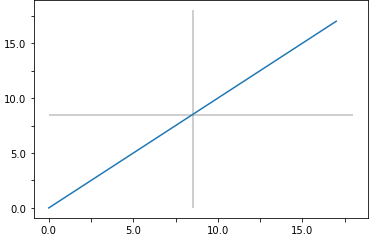
\includegraphics[width=0.5\linewidth]{linear}}
    \subfloat[$\omega(x)=((\frac{x+1}{p}) + 1)/2$]{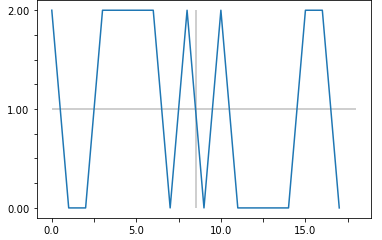
\includegraphics[width=0.5\linewidth]{legendre}}\\
    \caption{\footnotesize{Примеры антипалиндромических функций для $p=19$}}
\label{fig:antipalindromic}
\end{figure}

На \cref{fig:antipalindromic} показаны графики двух антипалиндромических функций. Для первой из них --- линейный функции $\omega(x)=x$ --- это свойство доказано выше. Вторая порождена символом Лежандра $(\frac{x+1}{p})$, её антипалиндромичность для простых чисел $p$ вида $4k+3$ является выражением свойства символа Лежандра и следует из закона квадратичной взаимности \cite{vinogradov}.

\section{Основная теорема о палиндромическом свойстве}
Следующая теорема даёт достаточное условие палиндромичности.

\begin{theorem}\label{palindromic_theorem}
Если функция $\omega$ антипалиндромическая, то заданный ей функционал $\psi$ обладает палиндромическим свойством.
\end{theorem}

Для доказательства теоремы понадобится следующая лемма:

\begin{lemma}\label{antipalindromic_lemma}
Пусть функционал $\psi$ задан антипалиндромической функцией. Тогда случайные последовательности $\{\psi(S^j x)\}_{j \ge 0}$ и $\{ \zeta - \psi(S^{-j} x)\}_{j \ge 0}$ равны по распределению. 
\end{lemma}
\begin{proof}
Прежде чем доказать лемму, приведём способ вычисления элементов данной последовательности.

Пусть $x \in \Gamma \setminus \{(p-1,p-1,\ldots)\}$ --- произвольный элемент. Определим порядок элемента $x$ как индекс его первой отличной от $p-1$ координаты: $\mathrm{order}(x) = k \ge 0$, если  $x_0=x_1=\ldots=x_{k-1}=p-1$ и $x_k \ne p-1$.

Рассмотрим последовательность $(\ldots, x-1,x,x+1, \ldots)$.  Легко видеть, что последовательность первых координат $(\ldots, (x-1)_0,x_0,(x+1)_0, \ldots)$ является периодической: в ней повторяется набор
$(0, 1, 2, \ldots,p-2, p-1$. Отсюда видно, что в исходной последовательности элементы порядка $0$ встречаются группами по $p-2$ элемента, между которыми находится ровно один элемент более высокого порядка (его первая координата $p-1$). Таким образом, последовательность
$\{\psi(S^j x)\}_{j \ge 0}$ состоит из блоков $\omega(0),\omega(1),\ldots, \omega(p-2)$, разделяемых одним элементом --- образом точки более высокого порядка. Чтобы найти недостающие элементы с индексами $j$, для которых $\mathrm{order}(S^j x) \ge 1$, отметим следующий факт. Если $x$ начинается с $p-1$, то для всех $j \ge 0$ выполнено $\psi(x+pj)=\psi(\sigma x + j)$. Следовательно, недостающие элементы последовательности соответствуют значениям $\{\psi(S^j \sigma x)\}_{j \ge 0}$. В свою очередь, для них верны приведённые выше рассуждения о последовательности первых координат: оказалось, что подпоследовательность с индексами, соответствующими элементам порядка $1$ и выше, повторяет всю исходную последовательность: она как бы вложена сама в себя.

Таким образом, мы можем построить всю последовательность $\{\psi(S^j x)\}_{j \ge 0}$ рекурсивно:
\begin{enumerate}
\item Выписываем значения для элементов порядка $0$ блоками $\omega(0),\omega(1),\ldots, \omega(p-2)$, разделяя их пропусками в один элемент. Мы выполняем циклический сдвиг блоков так, чтобы последовательность начиналась с $\omega(x_0)$, если $x$ --- элемент нулевого порядка, и с пропуска иначе.
\item Заполняем пропуски. Для этого рекурсивно запускаем процедуру для $x' = \sigma x$ и вписываем полученные элементы последовательно на места пропусков.

\begin{figure}[!h]
{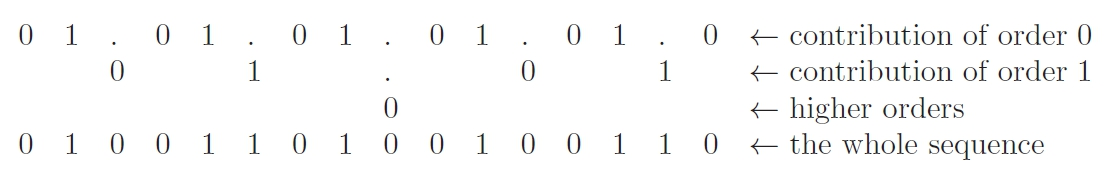
\includegraphics[width=\linewidth]{recursion}}
    \caption{\footnotesize{Пример построения последовательности $\{\psi(S^j x)\}$ для  $p=3$ и $x=0$ \cite{weaklimits}}}
\label{fig:psi_construction}
\end{figure}

\end{enumerate}

Перейдём к доказательству леммы. 

Заметим, что последовательность $\{ \zeta - \psi(S^{-j} x)\}_{j \ge 0}$ можно получить из $\{\psi(S^j x)\}_{j \ge 0}$ композицией двух сохраняющих меру преобразований:
\begin{enumerate}
\item Преобразование <<обращения>>  $\{a_j\}_{j \ge 0} \mapsto \{a_{-j}\}_{j \ge 0}$ 
\item Преобразование <<поэлементного дополнения>>, заменяющее каждый элемент $k \in \{b_j\}_{j \ge 0}$ на  $\zeta-k$; таким образом, получается последовательность $\{ \zeta - b_j\}_{j \ge 0}$ .
\end{enumerate}
По определению антипалиндромических функций, такое преобразование является тождественным для подпоследовательности элементов порядка $0$. В силу описанной выше конструкции, оно является тождественным для всей последовательности $\{\psi(S^j x)\}_{j \ge 0}$. Поскольку преобразование биективно и сохраняет меру, эти последовательности равны по распределению, что и требовалось доказать.
\bigskip\\
\end{proof}

Перейдём к доказательству теоремы.
\begin{proof}
В \cref{psi} подставим $\psi_\star = 0, \psi^\star = \delta = \zeta$. Достаточно показать, что  \[\forall j,\ 0 \le j \le m\zeta: \pi_m[\psi](j) = \pi_m[\psi](m \zeta - j).\]
Действительно,
$$\pi_m[\psi](m \zeta - j) = \lambda(\psi^{(m)}(x)=m\zeta-j)=$$ 
$$=\sum\limits_{(\psi_1, \ldots, \psi_m)} \lambda\big(\psi(x)=\psi_1, \psi^{(2)}(x) = \psi_2, \ldots, \psi^{(m)}(x)=\psi_m\big) \mathbb{I} (\psi_1 + \ldots + \psi_k = m\zeta - j) =$$
$$ = \sum\limits_{(\psi_1, \ldots, \psi_m)} \lambda\big(\psi(x)=\psi_1, \psi^{(2)}(x) = \psi_2, \ldots, \psi^{(m)}(x)=\psi_m\big) \mathbb{I} \big((\zeta-\psi_1) + \ldots + (\zeta-\psi_m) = j\big)$$
По предыдущей лемме это равно
$$\sum\limits_{(\psi_1, \ldots, \psi_m)} \lambda\big(\psi(x)=\zeta-\psi_m, \psi^{(2)}(x) = \zeta-\psi_{m-1}, \ldots, \psi^{(m)}(x)=\zeta-\psi_1\big) \mathbb{I} \big(\sum\limits_k (\zeta-\psi_k) = j\big) = \left< \psi_k := \zeta - \psi_k \right> =$$
$$ =\sum\limits_{(\psi_1, \ldots, \psi_m)} \lambda(\psi(x)=\psi_1, \psi^{(2)}(x) = \psi_2, \ldots, \psi^{(m)}(x)=\psi_m) \mathbb{I} (\psi_1 + \ldots + \psi_m = j) =  \lambda(\psi^{(m)}(x)=j)= $$
$$ =\pi_m[\psi](j)$$
\end{proof}

Результат этой теоремы может быть обобщён на более широкий класс функций. Фактически, мы сможем отказаться от ограничения на область значений функции $\omega$ в \cref{antipalindromic}.

\begin{corollary}\label{chacon_symmetry}
Коэффициенты характеристических полиномов обобщённого автоморфизма Шакона симметричны для любого $p \ge 3$ .
\end{corollary}
\begin{proof}
Отметим, что в соответствии с \cref{poly} коэффициентами полинома $P_m^p(t)$ являются значения $\pi_m(t)$. В силу \cref{palindromic} требование симметрии коэффициентов --- в точности то же самое, что палиндромическое свойство для $\phi$. В \cref{classic_omega} показали, что $\phi$ удовлетворяет условию \cref{palindromic_theorem}, и, следовательно, обладает палиндромическим свойством.
\end{proof}

Отдельный познавательный интерес представляет описание как можно более широкого класса функций, порождающих функционалы с палиндромическим свойством. Докажем несколько утверждений, обобщающих результат теоремы.

\begin{corollary}[Об аффинном преобразовании]
Пусть $\omega:[0,p-2] \rightarrow [0, \zeta]$ --- антипалиндромическая функция, тогда для любых $a > 0, b \ge 0$ функционал, заданный по правилу
$$\psi'(x) = \begin{cases}
                    a \omega(x_0) + b, & 0 \le x_0 \le p - 2 \\
                    \psi'(\sigma x), & x_0 = p - 1
                \end{cases}$$
обладает палиндромическим свойством.
\end{corollary}
\begin{proof}
Пусть $\pi_m'(j) = \lambda(\psi'^{(m)}(x)=j)$. В терминах \cref{antipalindromic}, $\psi_\star = b, \psi^\star = a\zeta + b, \delta = a\zeta$. Покажем, что $\pi_m'(mb + j) = \pi_m' (m(a\zeta+b)-j)$.

Выполним деление с остатком: $j = qa + r$. По построению $\psi'$ верно, что $\pi_m'(mb + qa + r) = 0$, если $r \ne 0$. Кроме того, $m(a\zeta+b)-j = m(a\zeta+b)-qa - r = mb + (m\zeta -q)a - r$, и следовательно, $\pi_m' (m(a\zeta+b)-j) = 0$, если $r \ne 0$.\\
Таким образом, достаточно показать, что $\pi_m'(mb + qa) = \pi_m' (m(a\zeta+b)-qa)$.
Заметим, что значения $\psi$, заданной функцией $\omega$, возможно восстановить из значений $\psi'$. Действительно, рассмотрим биекцию $i: \{b, a + b, 2a + b \ldots, a\zeta + b\} \rightarrow [0, \zeta]$, такую, что $i(j) = \frac{j-b}{a}$. Легко видеть, что $i(\psi'(x))=\psi(x)$. Аналогично, определим $i^{(m)}(j) = \frac{j-mb}{m}$ и получим $i^{(m)}(\psi'^{(m)}(x))=\psi(x)$. Отображение $i^{(m)}$ также является биекцией.

Теперь докажем, что $\pi_m'(mb + qa) = \pi_m' (m(a\zeta+b)-qa)$, пользуясь биективностью $i^{(m)}$.

\[\pi_m'(mb + qa) = \lambda(\psi'^{(m)}(x)=mb + qa) = \lambda\big(i^{(m)}(\psi'^{(m)}(x))=i^{(m)}(mb + qa)\big)  =\]\[= \lambda(\psi^{(m)}(x)= \frac{mb-qa-mb}{m})= \lambda(\psi^{(m)}(x)= q)=\pi_m(q)\]
Аналогично, $\pi_m' (m(a\zeta+b)-qa) = \pi_m(m\zeta - q)$. Так как $\omega$ --- антипалиндромическая функция, по \cref{palindromic_theorem} $\pi_m(q) = \pi_m(m \zeta - q)$, и следовательно $\pi_m'(mb + qa) = \pi_m' (m(a\zeta+b)-qa)$.
\end{proof}

Благодаря этому следствию мы можем показывать палиндромичность для достаточно большого класса функций. В частности, из этого следует, что если значения $\omega$ образуют арифметическую прогрессию, то она порождает палиндромический функционал. Действительно, любая такая функция получается аффинным преобразованием из антипалиндромической.

Отметим, что при доказательстве этого следствия мы не пользовались свойствами аффинного преобразования как такового. Фактически, оно является частным случаем более общего факта:
\begin{corollary}{О сохранении палиндромического свойства}
Пусть $\psi$ обладает палиндромическим свойством, и пусть функционал $\psi'$ таков, что для любого $m \in \mathbb{N}$ существует биекция $$i^{(m)}: \mathrm{Ran}\ \psi'^{(m)} \rightarrow \mathrm {Ran}\ \psi^{(m)}$$ Тогда $\psi'$ также обладает палиндромическим свойством.
\end{corollary}
Доказательство в точности повторяет рассуждения из предыдущей леммы. Важно, что рассматриваемая здесь биекция --- не просто соответствие значений $\omega$. Взаимная однозначность должна сохраняться для всех порядков $m$ функционала $\phi$, и это требование нельзя ослабить. В частности, преобразование $\omega(j) \mapsto \omega^2(j)$ является биекцией, но не сохраняет палиндромического свойства для задаваемых функционалов.
\chapter{Рекуррентные соотношения для характеристических полиномов}
В этой главе мы исследуем рекуррентные соотношения, которые позволят построить всё семейство характеристических полиномов алгебраически. Первый раздел посвящён выводу основных рекуррентных формул. Во втором разделе мы представим алгоритм вычисления характеристических полиномов и обсудим результаты.
\section{Вывод рекуррентных соотношений}
Для начала докажем простую лемму.

\begin{lemma}\label{simple_case} $P_{pm}^p(t)=t^{m\Delta_{p-2}}P_m^p(t)$
\end{lemma}
\begin{proof}
Пусть $x \in \Gamma'$. В соответствии с конструкцией для последовательности $\{\phi(S^j x)\}_{j \ge 0}$ (см. доказательство \cref{antipalindromic_lemma}), мы можем представить значение $\phi^{(pm)}(x)$ как сумму по порядкам аргумента: 
$$ \phi^{(pm)}(x) = \sum\limits_{\mathrm{order}(S^j x) = 0}^{0 \le j \le pm-1}\phi(S^j x) + \sum\limits_{\mathrm{order}(S^j x) \ge 1}^{0 \le j \le pm-1} \phi(S^j x)$$
\begin{itemize}
\item Найдём вклад в сумму элементов порядка $0$. Этих элементов ровно $(p-1)m$. Значения $phi$ на этих элементах вычисляются непосредственно по первой координате, так что они образуют периодическую последовательность $\ldots,(p-2),0,1,2,...,(p-2),0,1,\ldots$ Таким образом, сумма по элементам порядка $0$ распадается на $m$ одинаковых блоков, в каждом из которых встречаются по одному разу все числа отрезка $\left[ 0, p-2 \right]$. Их сумма равна $\Delta_{p-2}$, так что полный вклад элементов порядка $0$ составляет $\frac{(p-1)(p-2)}{2}m=m\Delta_{p-2}$
\item В соответствии с конструкцией из \cref{antipalindromic_lemma}, сумма по элементам порядка $1$ и выше в точности равна $\phi^{(m)}(\sigma x)$.
\end{itemize}
Итак, $\phi^{pm}(x) = m\Delta_{p-2} + \phi^{(m)}(\sigma x)$. По определению полиномов $P_m^p(t)$ отсюда следует 
$$P_{pm}^p(t) = \mathbb{E}_\lambda\left[ t^{\phi^{(pm)}(x)}\right] = 
\mathbb{E}_\lambda\left[ t^{m\Delta_{p-2} + \phi^{(m)}(\sigma x)}\right] = 
t^{m\Delta_{p-2}} \mathbb{E}_\lambda \left[ t^{\phi^{(m)} (\sigma x)}  \right] = 
t^{m\Delta_{p-2} }P_m(t)$$
\end{proof}

Данная лемма иллюстрирует метод, который будет использован для получения общего рекуррентного соотношения. Его вывод требует более глубокого комбинаторного рассмотрения сумм $\phi^{(pm+k)}(x)$, однако ход рассуждений останется в точности таким же.
\begin{lemma} \label{phiLemma}
Пусть $0 < k < p$,  $x=(x_0,x_1,\ldots) \in \Gamma'$.

$\phi^{(pm+k)}(x)= 
\begin{cases}
k x_0 + \Delta_{k-1} + m\Delta_{p-2} + \phi^{(m)}(\sigma x), & x_0 < p-k\\
(p-1-x_0)(x_0) + \Delta_{p-2-x_0} + \Delta_{x_0+k-p-1}+m\Delta_{p-2}+\phi^{(m+1)}(\sigma x), & x_0 \ge p-k
\end{cases}$
\end{lemma}
\begin{proof}
По определению $\phi^(k)$ выпишем $$\phi^{(pm+k)}(x) = \phi(x) + \phi(Sx) + \ldots + \phi(S^{k-1}x) + \phi^{(pm)}(S^k x)= \phi^{(k)}(x) + \phi^{(pm)}(S^k x)$$
По предыдущей лемме верно равенство $\phi^{(pm+k)}(x) =  \phi^{(k)}(x) + m\Delta_{p-2} + \phi^{(m)}(\sigma S^k x)$.
Пользуясь определением функционала $\phi(x)$, рассмотрим два случая, возникающих при вычислении $\phi^{(pm+k)}(x)$:
\begin{itemize}
\item В простом случае $x_0 < p-k $ каждое слагаемое в $\phi^{(k)}(x)$ вычисляется непосредственно по первой координате: $\phi^{(k)}(x) = k x_0 + \Delta_{k-1}$. Кроме того, имеет место равенство $\sigma S^k x = \sigma x$: так как $S^k$ действует только на первую координату $x$, его действие не влияет на $\sigma S^k x$. Итого, $$\phi^{(pm+k)}(x)=k x_0 + \Delta_{k-1}+m\Delta_{p-2}+\phi^{(m)}(\sigma x)$$
\item Пусть теперь $x_0 \ge p-k $, тогда одно из слагаемых в $\phi^{(k)}(x)$ вычисляется рекурсивно: для некоторого $j \in [0,k-1]$ элемент $S^j x$ имеет первую координату, равную $p-1$, и таким образом $\phi(S^j x) = \phi(\sigma x)$. Следовательно, значение $\phi^{(k)}(x)$ не может быть вычислено непосредственно, как в первом случае. Мы вычислим его, разделив сумму на две части. Сумма по начальному отрезку $\phi^{(p-1-x_0)}(x)$ может быть вычислена непосредственно и равна $(p-1-x_0)x_0 + \Delta_{p-2-x_0}$. Рассмотрим оставшуюся часть суммы $Z := \phi(S^j x) + \phi(S^{j+1}x) + \ldots + \phi(S^{k-1})$. По построению первая координата в $S^j x$ равна $p-1$, так что первые координаты следующих слагаемых $S^{j+1}x, S^{j+2}x, \ldots, S^{k-1}$ --- это числа $0,1,\ldots, x_0+k-p-1$. По определению $\phi(S^j x) = \phi(\sigma x)$, последующие слагаемые вычисляются непосредственно. Итого, $$Z = \phi(\sigma x) + 0 + 1 + \ldots + (x_0+k-p-1) =  \phi(\sigma x) + \Delta_{x_0+k-p-1}$$ Собирая полученные результаты, имеем $\phi^{(k)}(x)=\omega^{(p-1-x_0)}(x) + \Delta_{x_0+k-p-1}+\phi(\sigma x)$. Используя равенство $\phi^{(m)}(\sigma S^k x) = \phi^{(m)}(S\sigma x)  = \phi^{(m+1)}(\sigma x) - \phi(\sigma x)$, получим: 
$$\phi^{(pm+k)}(x) =  \phi^{(k)}(x) + m\Delta_{p-2} + \phi^{(m)}(\sigma S^k x) = $$ $$ = \omega^{(p-1-x_0)}(x) + \Delta_{x_0+k-p-1}+\phi(\sigma x)+ m\Delta_{p-2} + \phi^{(m+1)}(\sigma x) - \phi(\sigma x) = $$ $$ = (p-1-x_0)(x_0) + \Delta_{p-2-x_0} + \Delta_{x_0+k-p-1}+m\Delta_{p-2}+\phi^{(m+1)}(\sigma x)$$
\end{itemize}
\end{proof}

\begin{lemma} \label{complex_case}
Пусть $0 < k < p$.

$$P_{pm+k}^p(t)  =   \frac{1}{p} t^{m\Delta_{p-2} + \Delta_{k-1}}\sum\limits_{j=0}^{p-k-1} t^{jk} P_m^p(t) 
      + \frac{1}{p} t^{m\Delta_{p-2} + \Delta_{k-2}}\sum\limits_{j=0}^{k-1} t^{j(p-k)} P_{m+1}^p(t) $$
\end{lemma}
\begin{proof}
Доказательство заключается в разложении полного математического ожидания по условным. Ясно, что события $\{x_0 < p-k\}$ и $\{x_0 \ge p-k\}$ образуют полную систему событий. Их вероятности могут быть непосредственно вычислены по мере Хаара.
$$ P_{pm+k}(t)= \mathbb{E}_\lambda\left[ t^{\phi^{(pm+k)}(x)}\right] = $$
$$= \mathbb{E}_\lambda\left[ t^{\phi^{(pm+k)}(x)}| x_0 < p-k \right]\lambda(x_0<p-k) + \mathbb{E}_\lambda\left[ t^{\phi^{(pm+k)}(x)} | x_0 \ge p-k \right]\lambda( x_0 \ge p-k )$$
\begin{equation}\label{eq:totalExp}= \mathbb{E}_\lambda\left[ t^{\phi^{(pm+k)}(x)}| x_0 < p-k \right]\frac{p-k}{p} + \mathbb{E}_\lambda\left[ t^{\phi^{(pm+k)}(x)} | x_0 \ge p-k \right]\frac{k}{p}
\end{equation}
Условные математические ожидания, в свою очередь, могут быть вычислены с использованием результата предыдущей леммы. Заметим, что отдельные координаты $x$ как случайные величины независимы в совокупности, так что $x_0 \indep (x_1, x_2,\ldots)$ и, значит, $x_0 \indep \sigma x$. Вычислим первое условное математическое ожидание.
$$\mathbb{E}_\lambda\left[ t^{\phi^{(pm+k)}(x)}| x_0 < p-k \right] = 
\mathbb{E}_\lambda\left[ t^{ k x_0 + \Delta_{k-1} + m\Delta_{p-2} + \phi^{(m)}(\sigma x) }| x_0 < p-k \right] = $$ 
$$ =t^{m\Delta_{p-2}}
\mathbb{E}_\lambda\left[ t^{ k x_0 + \Delta_{k-1}} | x_0 < p-k \right]
 \mathbb{E}_\lambda\left[ t^{\phi^{(m)}(\sigma x) } \right]
$$
Случайные величины $\sigma x$ and $x$ распределены одинаково, так что
$\mathbb{E}_\lambda\left[ t^{\phi^{(m)}(\sigma x) } \right] = \mathbb{E}_\lambda\left[ t^{\phi^{(m)}(x) }\right] = P_m^p(t)$. Остаётся вычислить $\mathbb{E}_\lambda\left[ t^{ k x_0 + \Delta_{k-1}} | x_0 < p-k \right]$:
$$ \mathbb{E}_\lambda\left[ t^{ k x_0 + \Delta_{k-1}} | x_0 < p-k \right] =
 \frac{1}{p-k}\sum\limits_{j=0}^{p-k-1} t^{ k j + \Delta_{k-1}} = 
 \frac{1}{p-k} t^{\Delta_{k-1}}\sum\limits_{j=0}^{p-k-1} t^{kj}$$
 Итак, \begin{equation}\label{eq:firstCondExp}\mathbb{E}_\lambda\left[ t^{\phi^{(pm+k)}(x)}| x_0 < p-k \right] =
  \frac{1}{p-k} t^{m\Delta_{p-2} + \Delta_{k-1}}\sum\limits_{j=0}^{p-k-1} t^{jk} P_m^p(t)
   \end{equation}
Похожим образом вычислим второе условное матожидание. 
 $$\mathbb{E}_\lambda\left[ t^{\phi^{(pm+k)}(x)}| x_0 \ge p-k \right] = 
 \mathbb{E}_\lambda\left[ t^{(p-1-x_0)(x_0) + \Delta_{p-2-x_0} + \Delta_{x_0+k-p-1}+m\Delta_{p-2}+\phi^{(m+1)}(\sigma x)}| x_0 \ge p-k \right] = $$
 $$ =t^{m\Delta_{p-2}}
 \mathbb{E}_\lambda\left[ t^{(p-1-x_0)(x_0) + \Delta_{p-2-x_0} + \Delta_{x_0+k-p-1}} | x_0 \ge p-k \right] 
 \mathbb{E}_\lambda\left[ t^{\phi^{(m+1)}(\sigma x) } \right] = $$
  $$ =t^{m\Delta_{p-2}}
    P_{m+1}^p(t)
 \mathbb{E}_\lambda\left[ t^{(p-1-x_0)(x_0) + \Delta_{p-2-x_0} + \Delta_{x_0+k-p-1}} | x_0 \ge p-k \right] = $$
  $$ = \frac{1}{k} t^{m\Delta_{p-2}} P_{m+1}^p(t)
  \sum\limits_{j=p-k}^{p-1} t^{  (p-1-j) j + \Delta_{p-2-j} + \Delta_{j+k-p-1}}$$

Заменим индекс суммирования $j$ на $q = p-1-j$ и упростим выражение в показателе:
$$  (p-1-j) j + \Delta_{p-2-j} + \Delta_{j+k-p-1} =
    q(p-1-q) + \Delta_{q-1} + \Delta_{k-2-q}=
   q(p-k)+\Delta_{k-2} 
$$   
В итоге имеем: 
\begin{equation}\label{eq:secondCondExp}
\mathbb{E}_\lambda\left[ t^{\phi^{(pm+k)}(x)}| x_0 \ge p-k \right] 
 =  \frac{1}{k} t^{m\Delta_{p-2} + \Delta_{k-2}} P_{m+1}^p(t)
  \sum\limits_{q=0}^{k-1} t^{q(p-k)}
  \end{equation}
Подставим (\ref{eq:firstCondExp}) и (\ref{eq:secondCondExp}) в (\ref{eq:totalExp}) и получим рекуррентное соотношение:
$$P_{pm+k}(t)  =   \frac{1}{p} t^{m\Delta_{p-2} + \Delta_{k-1}}\sum\limits_{j=0}^{p-k-1} t^{jk} P_m^p(t) 
      + \frac{1}{p} t^{m\Delta_{p-2} + \Delta_{k-2}}\sum\limits_{j=0}^{k-1} t^{j(p-k)} P_{m+1}^p(t) $$
\end{proof}
\section{Вычисление характеристических полиномов}
Результаты \cref{simple_case} и \cref{complex_case} из предыдущего раздела объединим в теорему.
\begin{theorem}[Основные рекуррентные уравнения] 
\begin{align}
\label{P_pm} P_{pm}^p(t) & =  t^{m\Delta_{p-2}}\ P_m^p(t) \\
\label{P_pm+k} P_{pm+k}^p(t) & =  \frac{1}{p} t^{m\Delta_{p-2} + \Delta_{k-1}}\sum\limits_{j=0}^{p-k-1} t^{jk} P_m^p(t)  + \frac{1}{p} t^{m\Delta_{p-2} + \Delta_{k-2}}\sum\limits_{j=0}^{k-1} t^{j(p-k)} P_{m+1}^p(t), \ 0 < k < p
\end{align}
\end{theorem}
Для вычисления характеристических полиномов по этим соотношениям необходимы начальные условия. В Главе 1 мы уже получили первые два полинома $P_0^p(t)$ (\ref{eq:p_0}) и $P_1^p(t)$ (\ref{eq:p_1}). Покажем, что их достаточно для восстановления всего семейства. 

Действительно, зная $P_0^p(t)$ и $P_1^p(t)$, мы можем построить $P_2^p(t),\ \ldots
 ,\  P_{p-1}^p(t)$, воспользовавшись (\ref{P_pm+k}). Таким образом, нам известны полиномы $P_0^p(t)$ для всех $m < p$.
 
Отметим, что из полиномов для $m<p^k$ можно получить все полиномы для $p^k \le m < p^{k+1}$. Действительно, зафиксируем такое $m$. Выполним деление с остатком: $m = qp + r, \ p^{k-1} \le q < p^k,\ 0 \le r < p$. Если $r=0$, получаем нужный нам полином из уже известного $P_q^p(t)$ по формуле (\ref{P_pm}). Если $r \ne 0$, воспользуемся формулой (\ref{P_pm+k}), подставив в неё известные нам $P_q^p(t)$ и $P_{q+1}^p(t)$.

Таким образом, индукцией по степеням $p$ можно показать, что описанная процедура позволяет построить всё семейство полиномов $\{P_m^p(t)\}_m \ge 0$, зная только два начальных условия (\ref{eq:p_0}) и  (\ref{eq:p_1}).

В качестве примера выпишем первые несколько полиномов для небольших $p$. В таблице для каждого полинома $P_m^p$ указаны $d_m^p$ и $D_m^p$ --- минимальная и максимальная степень монома в полиноме, а так же унимодальность. 

\begin{table}[H]
\begin{small}
\begin{center}
\begin{tabular}{|c|c|c|c|c|c|}
\hline
$\mathbf{p}$ & $\mathbf{m}$& $\mathbf{P_m^p(t)}$ & $\mathbf{d_m^p}$ & $\mathbf{D_m^p}$& \textbf{ун.}\\
\hline
\multirow{10}{*}{3} & $1$ & $\frac{t}{2} + \frac{1}{2}$ & $0$  & $1$ & да \\
                    & $2$ &  $\frac{t^2}{6}+\frac{2 t}{3}+\frac{1}{6}$ & $0$ & $2$ & да \\
                    & $3$ &  $\frac{t^2}{2}+\frac{t}{2}$ & $1$ & $2$ & да \\
                    & $4$ &  $\frac{2 t^3}{9}+\frac{5 t^2}{9}+\frac{2 t}{9} $& $1$ & $3$ & да\\
                    & $5$ & $\frac{t^4}{18}+\frac{4 t^3}{9}+\frac{4 t^2}{9}+\frac{t}{18}$ & $1$ & $4$ & да \\
                   & $6$ & $\frac{t^4}{6}+\frac{2 t^3}{3}+\frac{t^2}{6}$ & $2$ & $4$ & да \\
                   & $7$ & $\frac{t^5}{18}+\frac{4 t^4}{9}+\frac{4 t^3}{9}+\frac{t^2}{18}$ & $2$ & $5$ & да \\
                   & $8$ & $\frac{2 t^5}{9}+\frac{5 t^4}{9}+\frac{2 t^3}{9}$ & $3$ & $5$ & да \\
                   & $9$ & $\frac{t^5}{2}+\frac{t^4}{2}$ & $4$ & $5$ & да \\
                   & $10$ & $\frac{13 t^6}{54}+\frac{14 t^5}{27}+\frac{13 t^4}{54}$ & $4$ & $6$ & да \\
\hline
\multirow{10}{*}{4} & $1$ & $\frac{t^2}{3}+\frac{t}{3}+\frac{1}{3}$ & $0$  & $2$ & да \\
                    & $2$ &  $\frac{t^4}{12}+\frac{t^3}{3}+\frac{t^2}{6}+\frac{t}{3}+\frac{1}{12}$ & $0$ & $4$ & нет \\
                    & $3$ &  $\frac{t^5}{12}+\frac{t^4}{6}+\frac{t^3}{2}+\frac{t^2}{6}+\frac{t}{12}$ & $1$ & $5$ & да \\
                    & $4$ &  $\frac{t^5}{3}+\frac{t^4}{3}+\frac{t^3}{3}$& $3$ & $5$ & да \\
                    & $5$ & $\frac{5 t^7}{48}+\frac{t^6}{4}+\frac{7 t^5}{24}+\frac{t^4}{4}+\frac{5 t^3}{48}$ & $3$ & $7$ & да\\
                    & $6$ & $\frac{t^9}{48}+\frac{t^8}{6}+\frac{7 t^7}{48}+\frac{t^6}{3}+\frac{7 t^5}{48}+\frac{t^4}{6}+\frac{t^3}{48}$ & $3$ & $9$ & да  \\
                    & $7$ & $\frac{t^{10}}{48}+\frac{5 t^9}{48}+\frac{11 t^8}{48}+\frac{7 t^7}{24}+\frac{11 t^6}{48}+\frac{5 t^5}{48}+\frac{t^4}{48}$ & $4$ & $10$ & да \\
                    & $8$ & $\frac{t^{10}}{12}+\frac{t^9}{3}+\frac{t^8}{6}+\frac{t^7}{3}+\frac{t^6}{12}$ & $6$ & $10$ & нет \\
                    & $9$ & $\frac{t^{12}}{48}+\frac{t^{11}}{8}+\frac{3 t^{10}}{16}+\frac{t^9}{3}+\frac{3 t^8}{16}+\frac{t^7}{8}+\frac{t^6}{48}$ & $6$ & $12$ & да \\
                    & $10$ & $ \frac{t^{13}}{24}+\frac{t^{12}}{8}+\frac{5 t^{11}}{24}+\frac{t^{10}}{4}+\frac{5 t^9}{24}+\frac{t^8}{8}+\frac{t^7}{24} $ & $7$ & $13$ & да \\
                    \hline
\multirow{10}{*}{5} & $1$ & $\frac{t^3}{4}+\frac{t^2}{4}+\frac{t}{4}+\frac{1}{4}$ & $0$  & $3$ & да \\
                    & $2$ &  $\frac{t^6}{20}+\frac{t^5}{4}+\frac{t^4}{20}+\frac{3 t^3}{10}+\frac{t^2}{20}+\frac{t}{4}+\frac{1}{20}$ & $0$ & $6$ & нет \\
                    & $3$ &  $\frac{t^8}{20}+\frac{t^7}{20}+\frac{3 t^6}{10}+\frac{t^5}{10}+\frac{t^4}{10}+\frac{3 t^3}{10}+\frac{t^2}{20}+\frac{t}{20}$ & $1$ & $8$ & нет \\
                    & $4$ &  $\frac{t^9}{20}+\frac{t^8}{10}+\frac{3 t^7}{20}+\frac{2 t^6}{5}+\frac{3 t^5}{20}+\frac{t^4}{10}+\frac{t^3}{20}$& $3$ & $9$ & да \\
                    & $5$ & $\frac{t^9}{4}+\frac{t^8}{4}+\frac{t^7}{4}+\frac{t^6}{4}$ & $6$ & $9$ & да\\
                    & $6$ & $\frac{3 t^{12}}{50}+\frac{3 t^{11}}{20}+\frac{4 t^{10}}{25}+\frac{13 t^9}{50}+\frac{4 t^8}{25}+\frac{3 t^7}{20}+\frac{3 t^6}{50}$ & $6$ & $12$ & да  \\
                    & $7$ & $\frac{t^{15}}{100}+\frac{t^{14}}{10}+\frac{3 t^{13}}{50}+\frac{17 t^{12}}{100}+\frac{4 t^{11}}{25}+\frac{4 t^{10}}{25}+\frac{17 t^9}{100}+\frac{3 t^8}{50}+\frac{t^7}{10}+\frac{t^6}{100}$ & $6$ & $15$ & нет \\
                    & $8$ & $\frac{t^{17}}{100}+\frac{t^{16}}{20}+\frac{7 t^{15}}{100}+\frac{4 t^{14}}{25}+\frac{2 t^{13}}{25}+\frac{13 t^{12}}{50}+\frac{2 t^{11}}{25}+\frac{4 t^{10}}{25}+\frac{7 t^9}{100}+\frac{t^8}{20}+\frac{t^7}{100}$ & $7$ & $17$ & нет \\
                    & $9$ & $\frac{t^{18}}{100}+\frac{3 t^{17}}{50}+\frac{7 t^{16}}{100}+\frac{9 t^{15}}{50}+\frac{9 t^{14}}{50}+\frac{9 t^{13}}{50}+\frac{9 t^{12}}{50}+\frac{7 t^{11}}{100}+\frac{3 t^{10}}{50}+\frac{t^9}{100}$ & $9$ & $18$ & да \\
                    & $10$ & $\frac{t^{18}}{20}+\frac{t^{17}}{4}+\frac{t^{16}}{20}+\frac{3 t^{15}}{10}+\frac{t^{14}}{20}+\frac{t^{13}}{4}+\frac{t^{12}}{20}$ & $12$ & $18$ & нет \\
\hline
\end{tabular}
\end{center}
\end{small}
\caption{\label{table:polynomials} Полиномы $P_m^p(t)$ для небольших $m$ и $p$.}
\end{table}

Отметим, что полученные формулы, как и ожидалось, согласуется с описанными в статье \cite{weaklimits} рекуррентными соотношениями для $p=3$. Подставив $p=3$ в (\ref{P_pm}) и (\ref{P_pm+k}) и раскрыв знаки суммирования, легко убедиться, что выполнены соотношения
\begin{align*}
P_{3m}^3(t) & =  t^{m}\ P_m^3(t) \\
P_{3m+1}^p(t) & =  \frac{1}{3} t^m (1 + t) P_m^3(t)  + \frac{1}{3} t^m P_{m+1}^3(t)\\
P_{3m+2}^p(t) & =  \frac{1}{3} t^m \cdot t\cdot  P_m^3(t)  + \frac{1}{3} t^m (1+t) P_{m+1}^3(t)
\end{align*}

\begin{definition} \nobreakspace\\
\begin{enumerate}
\item Числовая последовательность $\{a_n\}_{n \ge 0}$ называется унимодальной, если $\exists N \ge 0$, такое что $\{a_n\}_{0 \le n \le N}$ возрастает и $\{a_n\}_{n \ge N}$ убывает.
\item Дискретное распределение с вероятностями $(p_0,p_1,\ldots,p_n,\ldots)$ называется унимодальным, если его его вероятности образуют унимодальную последовательность.
\item Полином назовём унимодальным, если его коэффициенты в канонической форме образуют унимодальную последовательность.
\end{enumerate}
\end{definition}
Неформально, требование унимодальности означает наличие единственного максимума.
\begin{remark}
Унимодальность полинома $P_m^p(t)$ эквивалентна унимодальности распеределения с вероятностями $\pi_m$ для данного $p$.
\end{remark}

Отметим ещё одно важное следствие. В статье \cite{weaklimits} доказывалась унимодальность распределения $\pi_m$ при $p=3$. Далее это свойство сыграло значительную роль при доказательстве главного результата о слабых пределах. Однако легко видеть, что в общем случае распределение не унимодально. К примеру, полиномы $P_2^4$, $P_2^5$, $P_2^6$ не обладают унимодальными наборами коэффициентов. Более того, в силу соотношения (\ref{P_pm}) можно утверждать, что из существования хотя бы одного неунимодального полинома для данного $p$ следует существование бесконечного числа таких полиномов. С другой стороны, пользуясь начальным условием (\ref{eq:p_1}) и рассуждая аналогично, можно показать, что для любого $p$ существует бесконечно много унимодальных полиномов $P_m^p$.

\chapter{Степени полиномов. Симметризованная форма полиномов}
\section{Определения. Простые наблюдения}
Важным комбинаторным свойством рассматриваемого нами автоморфизма являются степени характеристических полиномов. Из \cref{poly} легко видеть, что каждая степень монома в полиноме $P_m^p(t)$ соответствует значению, которое достигается функционалом $\phi^{(m)}$ на некотором наборе элементов $\Gamma'$ с ненулевой вероятностной мерой. Дадим два важных определения.
\begin{definition}\label{high_deg}
Верхней степенью $D_m^p$ полинома $P_m^p(t)$ назовём максимальную степень входящего в него с ненулевым коэффициентом монома.
\end{definition}
\begin{definition}\label{low_deg}
Нижней степенью $d_m^p$ полинома $P_m^p(t)$ назовём минимальную степень входящего в него с ненулевым коэффициентом монома.
\end{definition}
Определение верхней степени в точности совпадает с алгебраическим определением \emph{степени полинома}.

Следующее утверждение устанавливает связь верхней и нижней степеней с областью значений функции\nobreakspace$\phi^{(m)}$.
\begin{proposition}
\begin{align*}
D_m^p &= \max\limits_{x \in \Gamma'} \phi^{(m)}(x)\\
d_m^p &= \min\limits_{x \in \Gamma'} \phi^{(m)}(x)
\end{align*}
\end{proposition}
\begin{proof}
Ввиду \cref{poly} утверждение почти очевидно. Остаётся показать, что все значения из $\mathrm{Im\ }\phi^{(m)}$ достигаются с ненулевой вероятностью.

Пусть $\phi_0 \in \mathrm{Im\ }\phi^{(m)}$. Тогда $\exists x \in \Gamma':\ \phi^{(m)}(x) = \phi_0$. Согласно \cref{phi} и \cref{phi_m} $\phi^{(m)}(x)$ зависит только от начальных координат $x$. Действительно, найдём $k$ --- максимальный среди элементов $x, Sx, S^2x, 
\ldots, S^{m-1}x$ индекс первой отличной от $p-1$ координаты. По определению множества $\Gamma'$ и оператора $S$ можно утверждать, что $k$ конечно. Ясно, что $\phi^{(m)}(x)$ зависит лишь от первых $k$ координат элемента $x$. Следовательно, зафиксировав эти первые $k$ координат и произвольно изменяя остальные, мы получим множество $X_{\phi_0}$ различных элементов $\Gamma'$, на которых $\phi^{(m)}$ принимает то же значение $\phi_0$. Вероятностная мера этого множества отделена от нуля: $$\lambda(X_{\phi_0}) = \frac{1}{p^k}$$
\end{proof}

Из формул (\ref{P_pm}), (\ref{P_pm+k}) видно, что и верхняя, и нижняя степени возрастают с ростом $m$. Это интуитивно ввиду аддитивного характера $\phi^{(m)}$. В частности, из указанных равенств и начального условия (\ref{eq:p_0}) непосредственно вытекает
\begin{align*}
d_{p^k}^p &= k \Delta_{p-2}\\
D_{p^k}^p &= k \Delta_{p-2} + p - 2
\end{align*}
Рост степеней полиномов делает менее явными некоторые комбинаторные, алгебраические и вероятностные свойства. Нижнюю степень $d_m^p$ можно интерпретировать как <<параметр сдвига>> распределения $\pi_m$. Этот сдвиг мешает сравнивать распределения друг с другом, выявлять их общие свойства. В частности, для каждого $m > 0$ полиномы $P_m^p, P_{2m}^p, \ldots, P_{km}^p,\ldots$ отличаются только множителем $t^{m\Delta_{p-2}}$, а соответствующие распределения --- сдвигом на $m\Delta_{p-2}$. 

Для анализа характера распределений возникает естественное желание избавиться от сдвига, привести все распределения к <<общему началу>>. В работе \cite{weaklimits} для этого предложена конструкция <<приведённых>> (англ. reduced) полиномов. Исходные полиномы делят на младшую степень: $$\tilde{P}_m^p(t) = t^{-d_m^p}P_m^p(t)$$
Легко видеть, что полученных полиномов степени начинаются с нуля. Это преобразование значительно упрощает работу с полиномами, однако его выполнение связано с технической сложностью. Далее будет показано, что нижние степени $d_m^p$ не могут быть записаны пригодной для вычисления замкнутой формулой, а следовательно, не могут быть получены и уравнения для вычисления приведённых полиномов.

В качестве альтернативы рассмотрим процедуру симметризации полиномов. Вместо деления на $t^{d_m^p}$ будем делить полиномы на $t^{\frac{d_m^p+D_m^p}{2}}$. Полученные выражения будут содержать степени $t$ от $-\frac{D_m^p - d_m^p}{2}$ до $\frac{D_m^p - d_m^p}{2}$ с шагом $1$. При чётном числе слагаемых степени $t$ будут полуцелыми, при нечётном --- целыми. Для каждого слагаемого с отрицательной степенью $t$ в полученное выражение входит слагаемое с противоположной степенью, причём в силу \cref{chacon_symmetry} они обладают равными коэффициентами. Таким образом, получается симметричное относительно нуля распределение коэффициентов.

\begin{definition}
Симметризованной формой полинома $P_m^p$ назовём выражение
$$ \SymPol{p}{m}(t) = t^{-\delta_m^p}P_m^p(t),$$
где $\delta_m^p=\frac{d_m^p+D_m^p}{2}$ --- средняя степень полинома $P_m^p$.
\end{definition}

В отличие от нижней степени, средняя степень $\delta_m^p$ легко поддаётся явному вычислению, что позволяет вывести для симметризованных форм рекуррентные уравнения, аналогичные (\ref{P_pm}) и (\ref{P_pm+k}).

Следующие разделы посвящены выводу выражения для средних степеней характеристических полиномов и рекуррентных уравнений для симметризованных форм.

\section{Последовательности $\hat{S}_j$ и $\hat{s}_j$}
Прежде чем перейти к изучению степеней характеристических полиномов, опишем две важных числовых последовательности. Их связь со степенями полиномов будет показана в следующем разделе.

\begin{definition}[Конструкция уровня $0$]
Положим $\hat{S}_0^{(0)} = p-2,\ \hat{S}_j^{(0)} = p-2-(j-1)$ for $j = \overline{1, p-1}$.
\end{definition}
Таким образом, получается последовательность $\{ \hat{S}_j^{(0)}\} = (p-2, p-2, p-3, \ldots, 2, 1, 0)$. 
\begin{definition} [Правило подстановки для $\{\hat{S}_j\}$]
Определим правило подстановки:
\begin{itemize}
 \item $0$ заменим на $p-2, p-3, \ldots, 2, 1, 0, 0$;
 \item $1$ заменим на $p-2, p-3, \ldots, 2, 1, 1, 0$;
 \item $2$ заменим на $p-2, p-3, \ldots, 2, 2, 1, 0$;
 \item \ldots
 \item $p-3$ заменим на $p-2, p-3, p-3, \ldots, 2, 1, 0$;
 \item $p-2$ заменим на $p-2, p-2, p-3, \ldots, 2, 1, 0$;
 \end{itemize}
\end{definition}
Таким образом, на место каждого числа $q \in [0, p-2]$ подставляется убывающая последовательность чисел от $p-2$ до $0$ с шагом $1$, где $q$ повторено дважды подряд.
\end{definition}
\begin{definition}[Конструкция уровня $1$]\label{tier1}
Выше была построена последовательность $\{ \hat{S}_j^{(0)}\}$  из $p$ элементов. Определим 
$\hat{S}_j^{(1)}$: заменим каждый элемент последовательности $\{ \hat{S}_j^{(0)}\}$ в соответствии с правилом подстановки. Так будет построена последовательность $\{\hat{S}_j^{(1)}\}$, состоящая из $p^2$ элементов.
\end{definition}
Продолжим процедуру: будем заменять каждый элемент $\{ \hat{S}_j^{(l)}\}$ по правилу подстановки и так получать $\{ \hat{S}_j^{(l+1)}\}$ . Легко видеть, что
\begin{itemize}
\item на каждом шаге длина последовательности увеличивается в $p$ раз
\item для каждого $l \ge 0$,  $\{ \hat{S}_j^{(l)}\}$ является начальным отрезком (префиксом) $\{ \hat{S}_j^{(l+1)}\}$.
\end{itemize}

Таким образом, начало последовательности стабилизируется. Существует последовательность $\{ \hat{S}_j^{(\infty)}\}$, в которой для каждого $l \ge 0$ последовательность $\{ \hat{S}_j^{(l)}\}$ содержится в качестве начального отрезка.
\begin{definition}
Let $\{\hat{S}_j\}_{j \ge 0} := \{ \hat{S}_j^{(\infty)}\}_{j \ge 0}$.
\end{definition}

\begin{remark}
Отметим, что аналогично можно определить данную последовательность, положив $\hat{S}_0 = p-2$ и применяя правило подстановки. Значит, последовательность однозначно определяется первым элементом. Этот факт будет использован далее.
\end{remark}
\begin{example}
Положим $p=4$. Выпишем первые уровни конструкции для $\hat{S}_j$.

$\begin{array}{|c|cccc|cccc|cccc|cccc|}
\hline
\{ \mathbf{\hat{S}_j^{(0)}}\} & 2 & & & & 2 & & & & 1 & & & & 0 & & & \\
\hline
\{ \mathbf{\hat{S}_j^{(1)}}\} & 2 & 2 & 1 & 0 & 2 & 2 & 1 & 0 & 2 & 1 & 1 & 0 & 2 & 1 & 0 & 0 \\
\hline
\{ \mathbf{\hat{S}_j^{(2)}}\} &
\text{\small{2210}} & \text{\small{2210}} & \text{\small{2110}} & \text{\small{2100}} &
\text{\small{2210}} & \text{\small{2210}} & \text{\small{2110}} & \text{\small{2100}} &
\text{\small{2210}} & \text{\small{2110}} & \text{\small{2110}} & \text{\small{2100}} &
\text{\small{2210}} & \text{\small{2110}} & \text{\small{2100}} & \text{\small{2100}} \\
\hline
 \mathbf{\ldots} & & & & & & & & & & & & & & & & \\
\hline
\end{array} $
\end{example}
\begin{proposition}[Характеристическое свойство для $\{\hat{S}_j\}$]\label{charProp}
Для любых $m > 0,\ 0 \le j \le p-1$ верно: 
\begin{equation}\label{eq:charProp}
\hat{S}_{pm+j}=\hat{S}_{p(p-1-\hat{S}_m) + j}
\end{equation}
\end{proposition}
\begin{proof}
Найдём наименьший уровень конструкции, на котором появляется $(pm+j)$-ый элемент последовательности: $l = \ceil{\log_p{m}}$. Этот $l$-ый уровень состоит из $p$ блоков, в каждом из которых $p^l$ элементов: каждый блок является подстановкой некоторого элемента предыдущего, $l-1$-ого элемента. В частности, элемент $\hat{S}_{pm+j}$ принадлежит блоку номер $m$ уровня $l$, полученному при подстановке $m$-ого элемента на уровне $l-1$. Следовательно,  
$\hat{S}_{pm+j}$ есть $j$-ый элемент в подстановке для $\hat{S}_m$.

Заметим, что все подстановки последовательно перечислены на уровне $1$, состоящем из элементов от $\hat{S}_0$ до $\hat{S}_{p^2-1}$. А именно, подстановка для элемента $q$ представлена элементами от $\hat{S}_{p + p(p-2-q)}$ до $\hat{S}_{p + p(p-2-q) + p-1}$. Чтобы получить $j$-ый элемент этой подстановки (считая с нуля 0), нужно найти $\hat{S}_{p + p(p-2-q) + j}$. 

Используя этот результат и упрощая выражение в индексе, получим, что $j$-ый элемент подстановки для $\hat{S}_m$ есть $\hat{S}_{p(p-1-S_m) + j}$, что доказывает требуемое утверждение.
\end{proof}
\begin{example}\label{Sj_evaluation}
Пусть $p=4$. Найдём $\hat{S}_{141}$.
$$ \hat{S}_{141} = \hat{S}_{4 \cdot 35 + 1} = \hat{S}_{4(3-\hat{S}_{35}) +1}$$
$$ \hat{S}_{35} = \hat{S}_{4 \cdot 8 + 3} = \hat{S}_{4(3-S_{8}) +3}$$
$$\hat{S}_8 = 2 \implies \hat{S}_{35}=\hat{S}_{4(3-2)+3}=\hat{S}_7=0$$
$$\hat{S}_{141}=\hat{S}_{4(3-\hat{S}_{35}) +1} = \hat{S}_{4(3-0)+1} = \hat{S}_{13}=1$$

\emph{Ответ:} 1.

\end{example}

Используя это свойство, можно дать более удобное эквивалентное определение для $\hat{S}$. Действительно, как показано в \cref{Sj_evaluation}, для любого $j \ge p^2$ можно найти элемент $\hat{S}_j$, применив формулу из \Cref{charProp} необходимое число раз. Таким образом, достаточно лишь определить конструкцию уровня $1$ (то есть значения элементов $\hat{S}_0, \ldots, \hat{S}_{p^2-1}$, чтобы построить всю последовательность с помощью этой формулы.
\begin{definition}\label{sm_good_def}
Определим $\{\hat{S}_j^{(1)}\}$ как в \Cref{tier1}. Положим
$$ \hat{S}_{pm+j} =
 \begin{cases}
     \hat{S}_{pm+j}^{(1)}, & m < p \\
     \hat{S}_{p(p-1-S_m) + j}, & m \ge p
 \end{cases}
$$
\end{definition}

Это определение будет использовано далее, чтобы показать связь $\{\hat{S}_j\}$ с верхними степенями полиномов.

Определим последовательность $\{\hat{s}_j\}$.
\begin{definition}
Пусть $j \ge 0$. Положим $\hat{s}_j = (p-2)-\hat{S}_j$
\end{definition}

Из данных выше определений следует, что $\{\hat{s}_j\}$ также является последовательностью, порождаемой подстановками.

\begin{proposition}[Правило подстановки для $\{\hat{s}_j\}$]
Последовательность $\{\hat{s}_j\}$ начинается с элемента $\hat{s}_0=0$ и подчиняется правилу подстановки:
\begin{itemize}
 \item $0$ заменим на $0, 0, 1, 2, \ldots, p-3, p-2$;
 \item $1$ заменим на $0, 1, 1, 2, \ldots, p-3, p-2$;
 \item $2$ заменим на $0, 1, 2, 2, \ldots, p-3, p-2$;
 \item \ldots
 \item $p-3$ заменим на $0, 1, 2, \ldots, p-3, p-3, p-2$;
 \item $p-2$ заменим на $0, 1, 2, \ldots, p-3, p-2, p-2$;
 \end{itemize}
\end{proposition}
\begin{proof}
В соответствии с предыдущим определением, достаточно выполнить замену $q' = p-2-q$ для всех чисел в правиле подстановки для $\{\hat{S}_j\}$ и найти $$\hat{s}_0 = p-2-\hat{S}_0 = p-2 - (p-2) = 0$$
\end{proof}

\begin{proposition}[Характеристическое свойство для $\{\hat{s}_j\}$]
Для любых $m > 0,\ 0 \le j \le p-1$ верно: $$\hat{s}_{pm+j}=\hat{s}_{p(1+\hat{s}_m) + j}$$
\end{proposition}
\begin{proof}
Подставим $\hat{S}_j = p-2-\hat{s}_j$ в (\ref{eq:charProp}):
$$p-2-\hat{s}_{pm+j}=p-2-\hat{s}_{p(p-1-(p-2-\hat{s}_m)) + j}$$
$$\hat{s}_{pm+j} = \hat{s}_{p(1+\hat{s}_m)+j}$$
\end{proof}

Последнее утверждение мы используем далее, чтобы показать связь $\{\hat{s}\}_j$ с нижними степенями характеристических полиномов.

\section{Рекуррентные соотношения для степеней полиномов}

\begin{proposition} \label{dm_eq}
Пусть $m \ge 0,\ 0 < k < p$. Тогда верны рекуррентные соотношения для верхних степеней:
\begin{align*}
  D_{pm}^p &= m \Delta_{p-2} + D_m^p \\
  D_{pm+k}^p &= m \Delta_{p-2}+(p-k)(k-1)+\Delta_{k-2}+D_m^p + \mathrm{max}\{p-k-1, D_{m+1}^p-D_m^p\}
\end{align*}
\end{proposition}
\begin{proof}
Непосредственно из (\ref{P_pm}) и (\ref{P_pm+k}) получим рекуррентные уравнения:
\begin{align*}
  D_{pm}^p &= m \Delta_{p-2} + D_m^p \\
  D_{pm+k}^p &= \mathrm{max}\{ m\Delta_{p-2} + \Delta_{k-1} + k(p-k-1) + D_m^p,\     
                                m\Delta_{p-2} + \Delta_{k-2} + (p-k)(k-1) + D_{m+1}^p \}
\end{align*}
Для доказательства утверждения достаточно вынести за знаки максимума общие слагаемые.
\end{proof}
Для дальнейших рассуждений зафиксируем произвольное $p \ge 3$.
\begin{definition} \label{sm_def}
Для каждого $m \ge 0$ положим $S_m := D_{m+1}^p - D_m^p $.
\end{definition}
Нам предстоит показать, что определённая таким образом последовательность $\{S_m\}_{m \ge 0}$ в точности совпадает с $\{\hat{S}_m\}$, описанной в предыдущем разделе. Для начала выведем рекуррентные соотношения на $S_m$.
\begin{proposition}
\begin{equation} \label{sm_eq}
S_{pm+k} = p-k-1 - \mathbbm{1}\{S_m < p-1-k\}
\end{equation}
\end{proposition}
\begin{proof}
Данное равенство доказывается при помощи \Cref{dm_eq} и \Cref{sm_def}. Возьмём произвольные $m$ и $k$ и вычислим $S_{pm+k}$. Возможны два случая:
\begin{itemize}
\item Пусть $k<p-1 $. $$S_{pm+k} = D_{pm+k+1}-D_{pm+k} =$$ $$= m\Delta_{p-2} + (p-k-1)k + \Delta_{k-1} + D_m + \max\{p-k-1, D_{m+1}-D_m\} - $$ $$ - m\Delta_{p-2}-(p-k)(k-1)-\Delta_{k-2}-D_m-\max\{p-k,D_{m+1}-D_m\}=$$ $$ =p-k-1+\max\{p-k-1, D_{m+1}-D_m\}-\max\{p-k,D_{m+1}-D_m\};$$
Подставим $D_{m+1}-D_m = S_m$ и заметим, что $$\max\{p-k-1, D_{m+1}-D_m\}-\max\{p-k,D_{m+1}-D_m\}= \mathbbm{1}\{S_m < 1-k\}.$$ Отсюда непосредственно получим требуемое равенство.
\item Разберём оставшийся случай: $S_{pm+p-1} = D_{p(m+1)}-D_{pm+3} = \\=(m+1)\Delta_{p-2}+D_{m+1}-m\Delta_{p-2}-(p-(p-1))(p-1-1)-\Delta_{p-1-2}-D_m-\max\{0, D_{m+1}-D_m\}=\\=\Delta_{p-2}+(D_{m+1}-D_m)-(p-2)-\Delta_{p-3}-(D_{m+1}-D_m)=0$
\end{itemize}

Непосредственная подстановка показывает, что второй случай подчиняется тому же равенству.
\end{proof}

\begin{lemma}\label{sm1}
Для всех $j = 0, 1, \ldots, p^2-1:\ S_j=\hat{S}_j^{(1)}$
\end{lemma}
\begin{proof}
Вычислим первые $p^2$ элементов последовательности $\{S_j\}$. Из начальных условий (\ref{eq:p_0}) и (\ref{eq:p_1}) получим $D_0 = 0,\ D_1 = p-2$, откуда по определению $S_0 = p-2$. Это равенство будем использовать как начальное условие для рекуррентного соотношения (\ref{sm_eq}).
Рассмотрим это соотношение. Правая часть состоит из двух слагаемых. Первое, $p-k-1$, является периодической функцией от $j$ с периодом, равным $p$, поскольку $k$ есть остаток от деления $j$ на $p$. Второе представляет собой функцию-<<ступеньку>> $-\mathbbm{1}\{S_m < p-1-k\}$, значение которой определяется номером периода. Таким образом, вычислим нужные элементы $\{S_j\}$ последовательно по периодам функции $p-k-1$.

Для первого периода $\{S_{0p+k}_{0 \le k < p}\}$ уже известно $S_0=p-2$. Слагаемое с индикатором здесь равно $-\mathbbm{1}\{k < 1\}$, так что оно обращается в нуль для каждого из $S_1, \ldots, S_{p-1}$. Они образуют убывающую последовательность $p-2, p-3, \ldots, 1, 0$. Таким образом, нам известны первые $p$ элементов $\{S_j\}$, которые тепепрь будут использованы для получения её дальнейших элементов.

Во втором периоде индикатор равен $\mathbbm{1}\{S_1 < p-1-k\}$. Поскольку $S_1=2$, второй период в точности повторяет первый. В третьем периоде индикатор равен $\mathbbm{1}\{S_1 < p-1-k\}=-\mathbbm{1}\{p-3 < p-1-k\} = -\mathbbm{1}\{k < 2\}$ и отличен от нуля только для первых двух элементов. Отсюда запишем элементы третьего периода: $p-2,p-3,p-3,p-4, \ldots, 1, 0$.

Аналогично, используем все элементы первого периода для вычисления $S_j$ для каждого $j < p^2$. 
Легко показать, что они в точности совпадают с элементами $\hat{S}_j^{(1)}$
\end{proof}

\begin{proposition} \label{sm_estimate}
$\forall j \ge 0:\ S_j \in \{0, 1, \ldots, p-2\}$
\end{proposition}
\begin{proof}
Вычислив $S_0, S_1, \ldots, S_{p-1}$, нетрудно убедиться в том, что
\begin{equation}\label{subset}
\{0,1,\ldots,p-2\} \subset \mathrm{Ran\ } \{S_j\}
\end{equation}

Очевидно, $\forall j \ge 0:\ S_j \ge 0$.
Покажем по индукции, что $\forall m \ge p,\ 0 < k < p-1:\ S_{pm+k} < p-1$. Параметром индукции будет служить <<номер порядка>> $\floor{\log_p m} =: u \ge 1}$. Прямое вычисление $S_p, S_{p+1}, \ldots, S_{p^2-1}$ доказывает базу индукции.

Докажем переход: пусть утверждение верно для некоторого $u \ge 1$. При вычислении элементов $S_j$ для порядка $u+1$ из уравнения (\ref{sm_eq}) мы используем значения элементов порядка $u$. В уравнении (\ref{sm_eq}) выполнено $p-k-1 \le p-1$ и $-\mathbbm{1}\{S_m < p-1-k\} \le 0$, так что $S_j \le p-1$. Покажем, что равенство никогда не достигается. Действительно, $p-k-1 = p-1$ верно лишь для $k=0$. Подставляя $k=0$ в индикатор, получим $- \mathbbm{1}\{S_m < p-1\}$. Для $S_m$ порядка $u$, неравенство в скобках истинно по предположению индукции. Таким образом, для порядка $u+1$ утверждение $S_j < p-1$ выполнено. Переход индукции доказан.

Теперь можно утверждать, что $\mathrm{Ran}\ \{S_j\} \subset \{0,1,\ldots,p-2\}$. Вместе с (\ref{subset}), это доказывает требуемое утверждение.
\end{proof}
\begin{lemma} \label{sm2}
Для всех $m \ge p,\ 0 < k < p-1:\ S_{pm+k}=S_{p(p-1-S_m)+k}$
\end{lemma}
\begin{proof}
Заметим, что для любого $j \ge 0$ выполнено $S_j = S_{p-1 - S_j}$. В силу \Cref{sm_estimate}, достаточно доказать утверждение для $S_j=0,1,\ldots,p-2$. Пусть, например, $S_j=0$. Легко проверить непосредственным вычислением, что $0 = S_{p-1}$. Аналогично утверждение проверяется для $S_j=1,\ldots,p-2$.

Докажем лемму. Пусть $m \ge p,\ 0 < k < p-1$. Из (\ref{sm_eq}) получим $S_{pm+k}=p-k-1 - \mathbbm{1}\{S_m < p-1-k\}$ и $S_{p(p-1-S_m)+k}= p-k-1 - \mathbbm{1}\{S_{p-1-S_m} < p-1-k\}$. Легко видеть, что равенство $S_m=p-1-S_m$ обращается в тождество.
\end{proof}
\begin{theorem} \label{subst_th}
Для любого $j \ge 0$: $S_j=\hat{S}_j$.
\end{theorem}
\begin{proof}
Утверждения \Cref{sm1} и \Cref{sm2} означают, что \Cref{sm_good_def} верно для $\{S_j\}_{j \ge 0}$.
\end{proof}
\begin{corollary}
$$D_m = \sum\limits_{j=0}^{m-1} \hat{S}_j$$
\end{corollary}


\chapter{Моделирование данных и статистик}

Покажем на экспериментальных примерах, что статистика $\hat{a}$ имеет основания быть состоятельной и асимпотически нормальной. Для этого расмотрим следующие примеры распределений:
\begin{enumerate}
  \item $X_l \sim \mathcal{N}(10, 1)$, параметр сдвига $a = 10$ (рис. \textit{fig:normshift}).
  \item $X_l \sim Exp(1)$ с параметром сдвига $a = 5$ (рис. \textit{fig:expshift}).
\end{enumerate}
В ходе каждого эксперимента, сгенерируем 1000 выборок размера $n = 1000000$, зададим величину $1 \le k_n \le 1000 = \sqrt{n}$, и рассмотрим графики поведения среднего значения статистики $\hat{a}_{\max}$ в зависимости от $k$, гистограммы поведения статистики при $k = 1000$.

%\begin{figure}[!h]
%    \subfloat[Гистограмма]{\includegraphics[width=0.5\textwidth]{./norm_hist_shift.eps}}
%    \subfloat[Значение $\hat{a}_{\max}$]{\includegraphics[width=0.5\textwidth]{./norm_mean_shift.eps}}\\
%    \caption{\small Данные по выборке из нормального распределения, параметр сдвига $a = 10$}
%    \label{fig:norm_shift}
%\end{figure}

%\begin{figure}[!h]
 %   \subfloat[Гистограмма]{\includegraphics[width=0.5\textwidth]{./exp_hist_shift.eps}}
%    \subfloat[Значение $\hat{a}_{\max}$]{\includegraphics[width=0.5\textwidth]{./exp_mean_shift.eps}}\\
%    \caption{\small Данные по выборке из экспоненциального распределения, параметр сдвига $a = 5$}
%    \label{fig:exp_shift}
%\end{figure}


Из представленных графиков видно, что в рассмотренных распределениях гистограмма похожа на график плотности нормального распределения, а среднее значение сходится к истинному значению параметра, поэтому статистика $\hat{a}_{\max}$ может быть подвергнута дальнейшему исследованию.



Аналогично предыдущему случаю, построим графики и гистограммы для следующих распределений:

\begin{enumerate}
  \item $X_l \sim \mathcal{N}(5, 25)$, параметр масштаба $b = 5$,
  \item $X_l \sim Exp(10)$ с параметром масштаба $b = 10$,
  \item $X_l \sim Pareto(1.2)$, параметр масштаба $b = 10$.
\end{enumerate}


%\begin{figure}[!h]
%    \subfloat[Гистограмма]{\includegraphics[width=0.5\textwidth]{./norm_hist_scale.eps}}
%    \subfloat[Значение $\hat{b}_{\max}$]{\includegraphics[width=0.5\textwidth]{./norm_mean_scale.eps}}\\
%    \caption{\small Данные по выборке из нормального распределения, параметр $b = 5$}
%    \label{fig:norm_scale}
%\end{figure}

%\begin{figure}[!h]
%    \subfloat[Гистограмма]{\includegraphics[width=0.5\textwidth]{./exp_hist_scale.eps}}
%    \subfloat[Значение $\hat{b}_{\max}$]{\includegraphics[width=0.5\textwidth]{./exp_mean_scale.eps}}\\
%    \caption{\small Данные по выборке из экспоненциального распределения, параметр $b = 10$}
%    \label{fig:norm_scale}
%\end{figure}


%\begin{figure}[!h]
%    \subfloat[Гистограмма]{\includegraphics[width=0.5\textwidth]{./pareto_hist.eps}}
%    \subfloat[Значение $\hat{b}_{\max}$]{\includegraphics[width=0.5\textwidth]{./pareto_mean.eps}}\\
%    \caption{\small Данные по выборке из распределения Парето, параметр $b = 10$}
%    \label{fig:pareto_scale}
%\end{figure}


Как и в предыдущем случае, гистограммы оценок параметра масштаба для $k = 1000$ похожи на гистограммы плотности нормального распределения.

\newpage
\bibliography{chacon}


\end{document}
